\subsection{Bedienung des Editors}
Der Editor ist über den Text, Draw, Shape oder Image Button erreichbar. Öffnet man zum ersten Mal den Editor, so wird initial der Text Button des Hauptmenüs ausgewählt. Befindet man sich im Editor, so kann man dann auch Draw, Shape oder Image selektieren. Genau wie im Reader erscheint zuerst ein Button Choose file. Je nachdem ob man nach erstmaligem Öffnen einer PDF-Datei auf Text, Draw, Shape oder Image geklickt hat, wird als erstes der Writer, Drawer, Geometry oder Image Bearbeitungsmodus des jeweiligen Editormoduls geöffnet. Hat man eine Datei geöffnet, so befindet sich der Reader ohne die Operationen zum Seiten Drehen ebenfalls in jedem Editormodul. Alle input fields im Editor sind mit dem gültigen Wertebereich für Benutzereingaben als Information Min: Max: versehen. Der Editor samt dargestellter PDF-Datei besteht aus einem grauen waagerechten Operations Bar, einem linken Ebenen Seitenmenü in Rosa und einem rechten grünen Tools Seitenmenü. Mit dem ganz linken grünen Button Layers im Operations Bar kann das Ebenen Seitenmenü aus- und eingeblendet werden. Daneben zeigt oder verbirgt der Button Tools das Tools Seitenmenü. Standardmäßig sind die Ebenen und Tools Seitenmenüs ausgeklappt. 

\subsubsection{Textbearbeitung}
Hat man den Writer aufgerufen, so präsentiert sich einem der Texteditor in den folgenden Abbildungen \ref{fig:texteditor} und \ref{fig:texteditor2}.

\begin{figure}[!htbp]
	\centering
	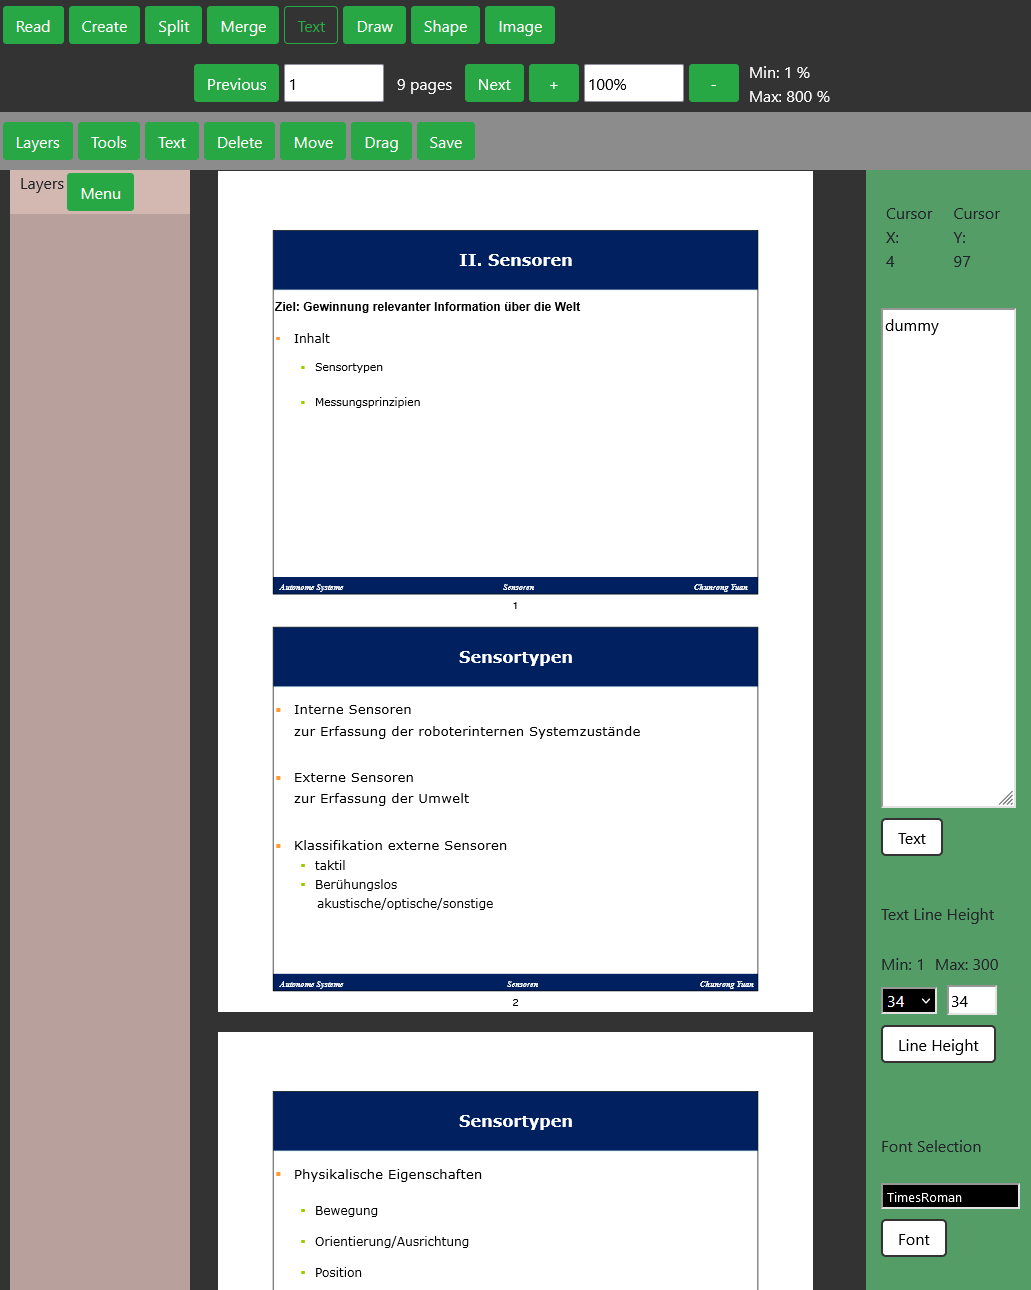
\includegraphics[width=1\textwidth]{"images/texteditor.png"}
	\caption{Startseite des Texteditors der PDF Web App}
	\label{fig:texteditor}
\end{figure}

\begin{figure}[!htbp]
	\centering
	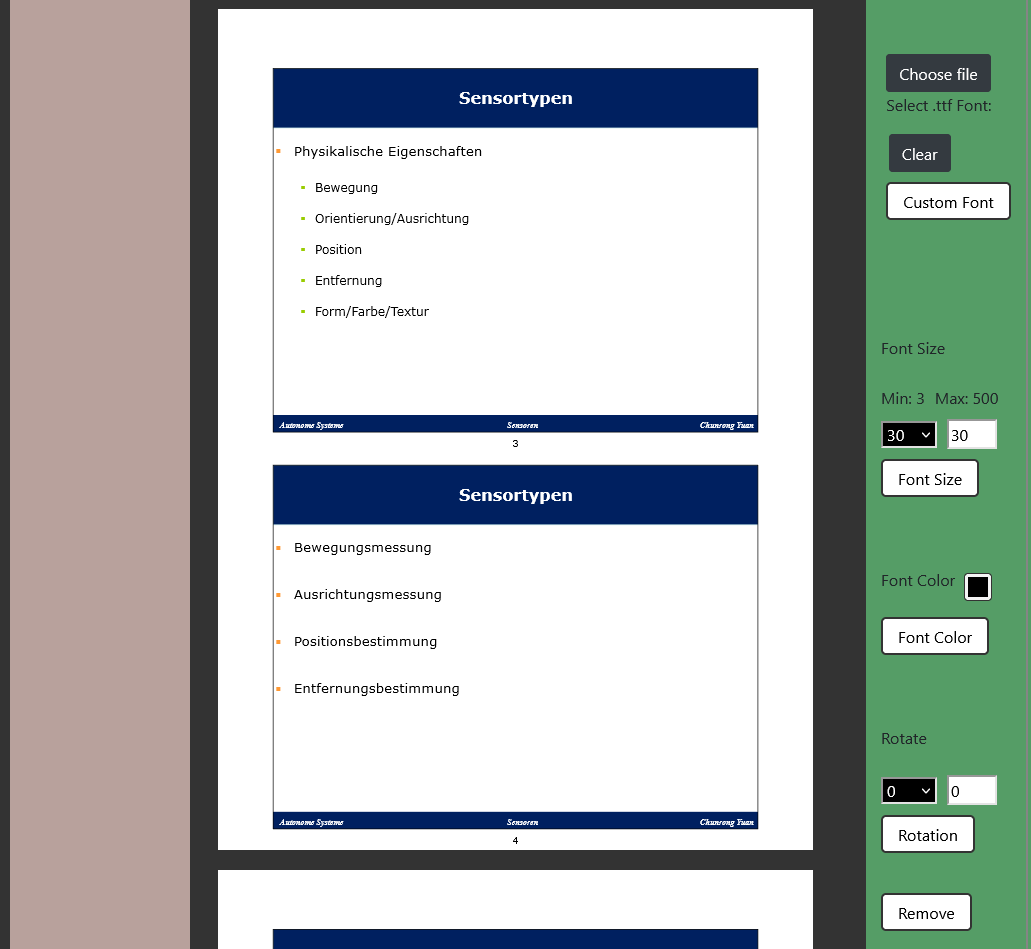
\includegraphics[width=1\textwidth]{"images/texteditor2.png"}
	\caption{Mehr Tools der Startseite des Texteditors der PDF Web App}
	\label{fig:texteditor2}
\end{figure}

Mit dem Button Text in dem Operations Bar und nachfolgendem Klick aufs geöffnete Dokument kann man einen Text mit dem Platzhaltertext dummy hinzufügen. Unter dem Text erscheint eine dunkelrote control box, auf die man alle Operationen im Operations Bar und dem Tools Seitenmenü im Box Mode anwenden kann. Ich werde zunächst alle Operationen im Box Mode beschreiben und später auf den Layer Mode eingehen. Der Box Mode ist standardmäßig eingestellt. Operationen können durch die grünen Buttons zum Erstellen neuer Elemente, Delete oder Move im Operations Bar und allen weißen Buttons im Tools Seitenmenü getriggert werden. Hat man eine Operation getriggert, so befindet man sich im Modus dieser Operation im Box Mode und man kann darauffolgend in alle im Dokument verfügbaren control boxes sämtlicher Elementtypen klicken, um die Operation auf das betreffende Element auszuführen. Das bedeutet außerdem, dass man in jedem Editormodul nur neu hinzugefügte Elemente editieren und nicht bereits im geöffneten Dokument eingebettete Objekte verändern kann. Alle Operationen im rechten Tools Seitenmenü beziehen sich jeweils auf das Element des aktuellen Editormoduls und sind nur auf diesem anwendbar. In der Praxis bedeutet das, dass man mehrere Texte, ohne erneut den grünen Text Button drücken zu müssen, dem PDF-Dokument hinzufügen kann. Für jedes neu hinzugefügte Editorelement wird eine Ebene mit einem elementspezifischen Standardnamen erstellt, die im linken rosa Ebenenmenü erscheint. Die obere linke Ecke der quadratischen control box sämtlicher Editorelemente wird generell dort platziert, wo man mit der Maus auf die Seite geklickt hat. Alle control boxes werden nicht im  Output PDF gespeichert, denn sie dienen lediglich der Steuerung von Editorelementen, um Operationen im Box Mode anwenden zu können. Mit dem Delete Button und nachfolgendem Klick in eine oder mehrere control boxes im Box Mode können Texte wieder gelöscht werden. Move verschiebt einzelne Texte durch eine mit der Maus gedrückte und zur Zielposition bewegte control box. Wenn die Maus losgelassen wird, nachdem die control box verschoben wurde, springt der Text an die Zielposition auf der PDF-Seite. Delete und Move kommen in allen Editormodulen vor und funktionieren immer gleich. Jedoch wirken sich Delete und Move nur auf die im jeweiligen Editor zu bearbeitenden Elemente aus. Ganz oben im Tools Seitenmenü werden dem Betrachter die x- und y-Koordinaten des Mauscursors auf der PDF Seite angezeigt, wenn die Maus über eine Seite bewegt wird. Diese Mauscursorkoordinaten kommen in jedem Editormodul vor. Darunter kann man in der textarea den Text editieren. Es werden auch Zeilenumbrüche berücksichtigt. Nachdem man den dummy Text in der textarea überschrieben hat, einem Klick auf den weißen Text Button und der Anwendung auf control boxes, wir der Platzhaltertext mit dem aktuellen Text in der textarea substituiert. Alle Operationen in Tools in allen Editormodulen werden genau gleich ausgeführt: Man tätigt seine Einstellung, drückt mit der linken Maustaste auf den weißen Button für die jeweilige Operation und klickt daraufhin auf ein oder mehrere control boxen von Elementen nacheinander. Unterhalb der Texteditierungsoperation kann man den Zeilenabstand einstellen. Entweder verwendet man das selection menu mit voreingestellten Werten oder man gibt einen gewünschten Wert manuell in das input field ein. Alle selection Menüs und input fields in jedem Editormodul zeigen die default Werte, mit denen ein neu hinzugefügtes Element konfiguriert ist, an. Falls man zuletzt das selection Menü betätigt hat, überschreibt es den im input field befindlichen Wert und umgekehrt. Maßgeblich ist, was man zuletzt betätigt hat. Dieses Verhalten habe ich bei jeder selection menu und input field Kombination programmiert. Einen benutzerdefinierten TrueType-Font kann man durch den dunkelgrauen Choose file Button vom Dateisystem auswählen und er erscheint in einer Liste. Der zuletzt geöffnete Font wird ausgewählt. Mittels Clear kann man alle Fonts aus der Liste entfernen, was nicht heißt, dass sie auch auf den angewendeten Textelementen entfernt werden. Abbildung \ref{fig:custom-font} zeigt 2 geöffnete .ttf Schriftdateien in der Liste.

\begin{figure}[!htbp]
	\centering
	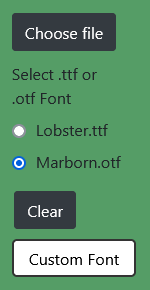
\includegraphics[width=0.3\textwidth]{"images/custom-font.png"}
	\caption{Benutzerdefinierte Fontliste im Texteditor der PDF Web App}
	\label{fig:custom-font}
\end{figure}

Die Fontgröße kann man ebenfalls wie die Zeilenhöhe mit selection menu und input field justieren. Bei der Fontfarbe klickt man auf das initial schwarze Quadrat, was die aktuelle Farbe zeigt, und es öffnet sich ein color picker menu. Hier kann man die Farbe und Transparenz einstellen. Die Farbwerte kann man sich in RGBA, HSLA oder HEX formatieren lassen. Mit Klick auf die beiden kleinen senkrechten Pfeile im color picker wird jeweils das Format gewechselt. Das Fenster des color pickers für die Fontfarbe ist in Abbildung \ref{fig:fontcolor} abgebildet. 

\begin{figure}[!htbp]
	\centering
	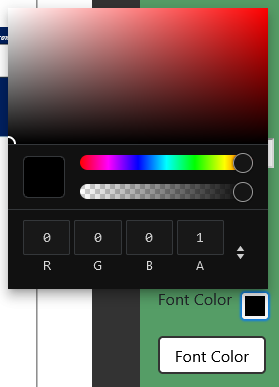
\includegraphics[width=0.5\textwidth]{"images/fontcolor.png"}
	\caption{Color picker für die Fontfarbe des Texteditors der PDF Web App}
	\label{fig:fontcolor}
\end{figure}

Als vorletzte Option kann man den Text absolut drehen. Durch den weißen Button Rotation und der entsprechenden Benutzerinteraktion durch selection Menu oder input field wird das Textelement rotiert. Absolute Rotation bedeutet, dass es eine feste Rotationsskala gibt anhand der das Element rotiert wird. Folglich passiert keine Veränderung, wenn man den gleichen Rotationswert 2 Mal hintereinander ausführt. Stellt man einen Rotationswinkel von 0 Grad ein, so wird das Element wieder zurück auf die Ausgangsrotation bei Erstellung gedreht. Alle Editormodule verwenden absolute Rotation. Abschließend können alle Textelemente im Dokument mit dem Remove Button auf einen Schlag gelöscht werden. Beim Zeilenabstand und der Schriftgröße wird der Benutzer außerdem über den Wertebereich von Benutzereingaben informiert. Die Textoperationen werden in Abbildung \ref{fig:text} demonstriert.

\begin{figure}[!htbp]
	\centering
	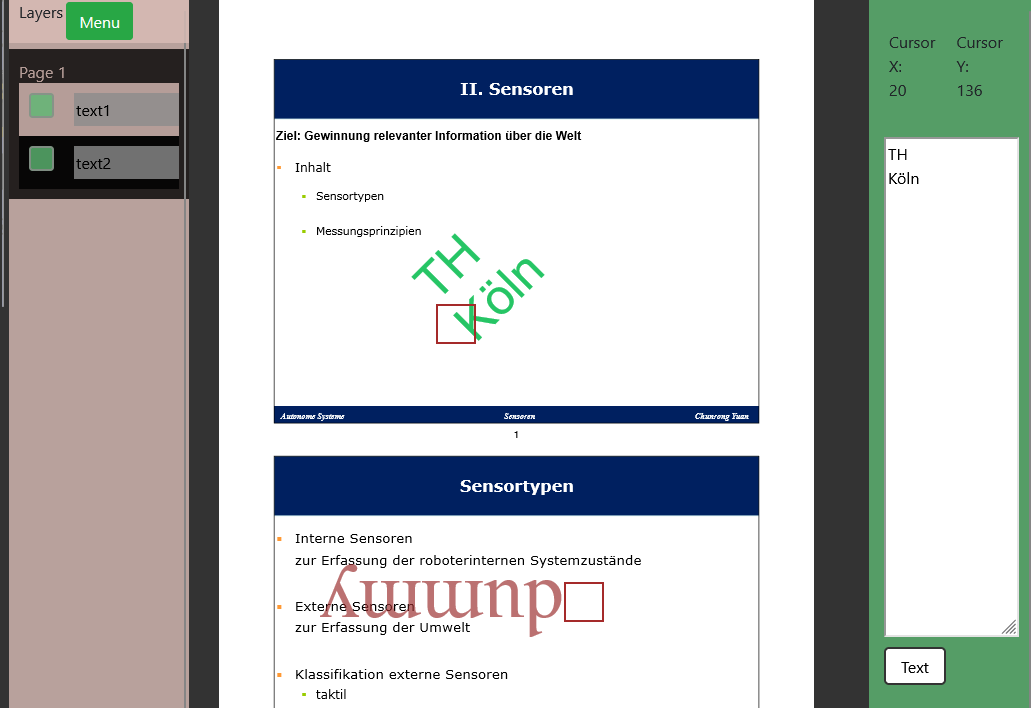
\includegraphics[width=0.9\textwidth]{"images/text.png"}
	\caption{Bearbeiteter Text im Writer der PDF Web App}
	\label{fig:text}
\end{figure}

\subsubsection{Zeichnungen erstellen}
Der Drawer ist in Screenshot \ref{fig:drawer} abgebildet. 

\begin{figure}[!htbp]
	\centering
	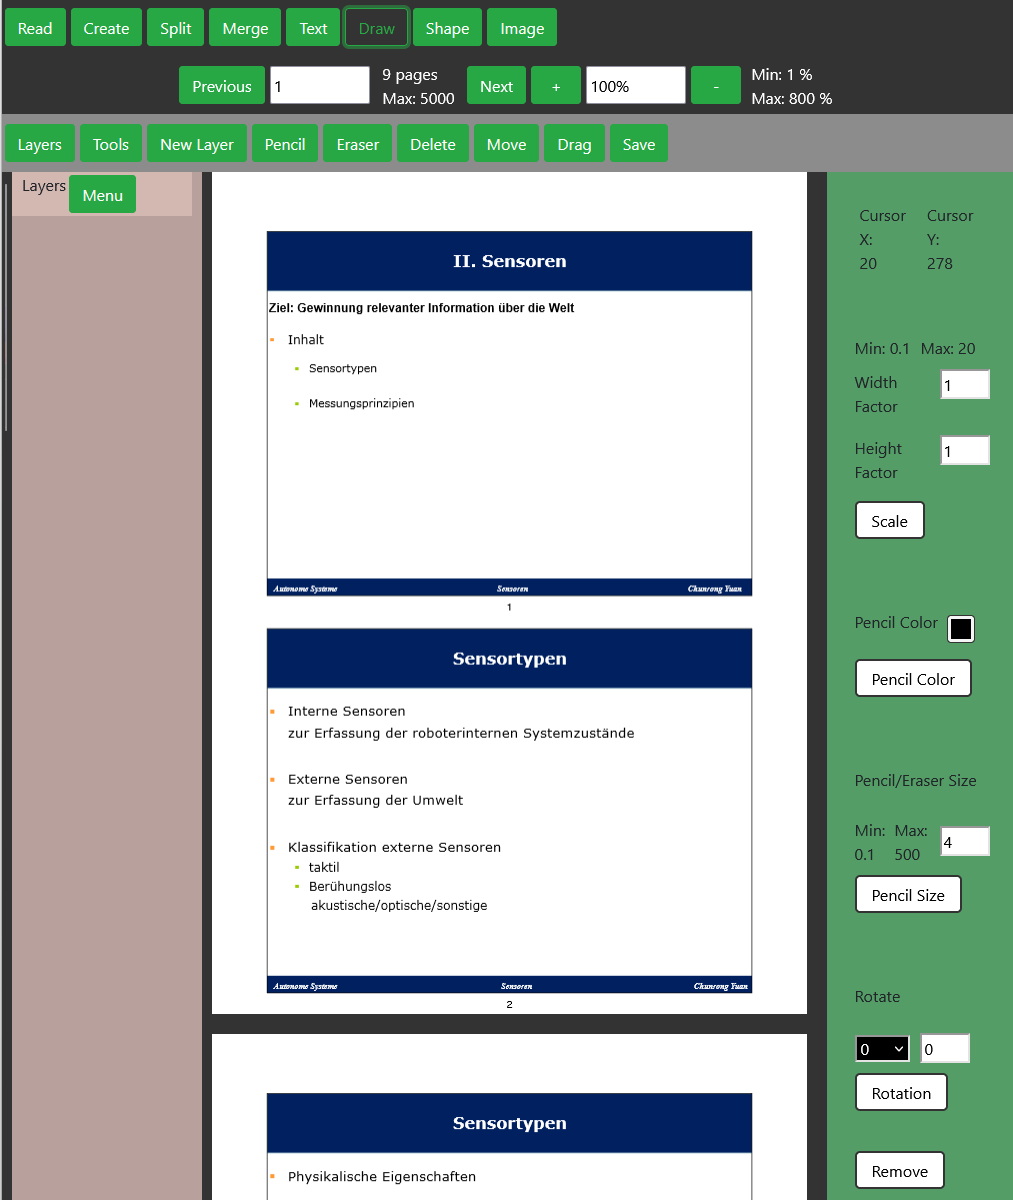
\includegraphics[width=1\textwidth]{"images/drawer.png"}
	\caption{Drawer der PDF Web App}
	\label{fig:drawer}
\end{figure}

Das Ebenenmenü und Tools Seitenmenü des Drawers erscheint selbst, wenn man zuerst in einem anderen Editormodul ein Dokument geöffnet hat. Generell braucht man nur einmalig ein PDF zu öffnen und kann dann in die jeweiligen Bearbeitungsmodi jedes Editormoduls wechseln. Um ein neues PDF zu öffnen kann man entweder die PDF Web App neu laden oder man klickt erst auf Read, Create, Split oder Merge und anschließend wieder auf ein Editormodul, damit der Choose file Button erneut angezeigt wird. Mit dem Zeichnen kann man beginnen, indem man auf Pencil klickt. Bei gedrückter Maustaste auf einer PDF Seite erscheint eine schwarze Linie dort wo die Maus sich bewegt hat. Zusätzlich wird an der Stelle, wo man angefangen hat die Maus zu drücken, eine Magenta farbige control box hinzugefügt. Das Zeichnen funktioniert auch mit einem Graphic Tablet. Es wird immer auf der zuletzt gezeichneten Ebene auf der zugehörigen Seite gemalt bzw. wenn man eine Ebene auswählt im Ebenen Seitenmenü wird auf der ausgewählten Ebene gezeichnet. Ein Klick auf New Layer und anschließender Zeichenmodus mit Pencil erstellt für die neue Zeichnung eine weitere Ebene. Wurde auf einer Seite bisher noch nichts gezeichnet, so wird bei der ersten Zeichnung auf dieser Seite eine neue Ebene automatisch angelegt und man muss dafür nicht New Layer drücken. Die Zeichenelemente sind die einzigen Elemente, bei denen der Nutzer selbst die Ebenen einer Seite zuweisen kann mit New Layer. Bei allen anderen Elementen, sei es Text, Geometrie oder Bilder, wird  jedes neue Element automatisch einer Ebene zugeteilt. Der Radierer ist mit dem Eraser Button Operations Bar aufrufbar. Zuerst drückt man Eraser und geht dann mit gedrückter Maustaste über die Zeichnungen auf einer Seite, die man entfernen möchte. Auch hier gilt, das auf der ausgewählten Ebene radiert wird. Dort, wo bei gedrückter Maustaste die Maus die Linie berührt, wird die Linie wegradiert. Zeichnen und Radieren bekommen jeweils ein neues Mauscursorsymbol: Beim Zeichnen hat man ein schwarzes dünnes Kreuz und beim Radieren ein weißes dickes Kreuz. Im Tools Seitenmenü kann man eine Zeichnung relativ skalieren, indem man einen Faktor eingibt. Der Faktor kann auch ein Float sein und multipliziert sich immer mit der aktuellen Größe, d.h. die aktuelle Größe wird als 100 \% berechnet. Darunter kann man mit dem color picker menu die Farbe und Transparenz der Stiftfarbe definieren. Sie wird mit einem Klick auf Pencil Color auf die nächste Zeichenoperation angewendet. Außerdem definiert sie auch gleichzeitig die Radiererfarbe, was sich nur bei Transparenzen unter einem Wert von 1 bemerkbar macht. Ansonsten ist jede Radiererfarbe gleich, jedoch bei einer Transparenz von unter 1 radiert der Radierer weniger deckend, so als ob man einen Radiergrummi weniger stark auf das Papier drückt. Dann kann man die Größe des Stiftes bzw. Radierers einstellen. Sie greift auch ab der nächsten Zeichnen- bzw. Radieroperation. Ebenfalls kann man Zeichnungen samt radierten Partien rotieren. Zum Schluss kann man mit Remove alle Zeichnungen im Dokument löschen. Teilweise transparente Zeichnungen werden im Bild \ref{fig:drawing} dargestellt. 

\begin{figure}[!htbp]
	\centering
	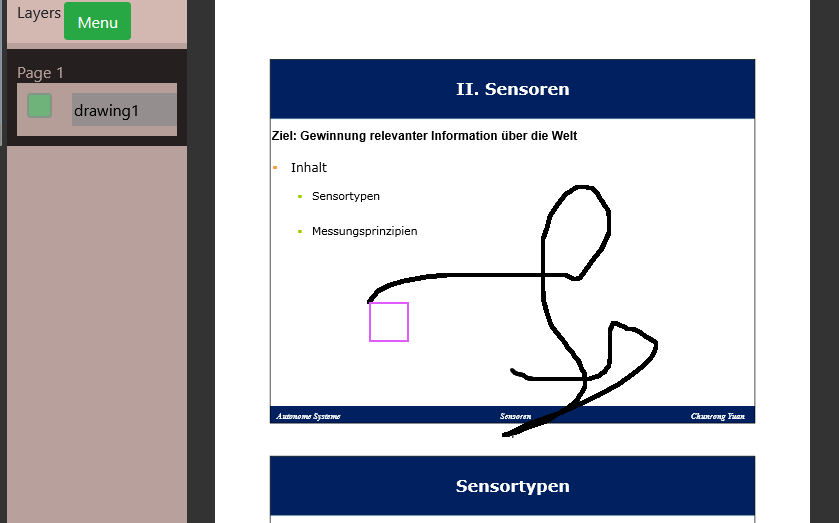
\includegraphics[width=1\textwidth]{"images/drawing.png"}
	\caption{Zeichnungen im Drawer der PDF Web App}
	\label{fig:drawing}
\end{figure}


\subsubsection{Geometrie hinzufügen}
Die Startseite des Geometry Editor ist in den Screenshots \ref{fig:shaper} und \ref{fig:shaper2} abgebildet. 

\begin{figure}[!htbp]
	\centering
	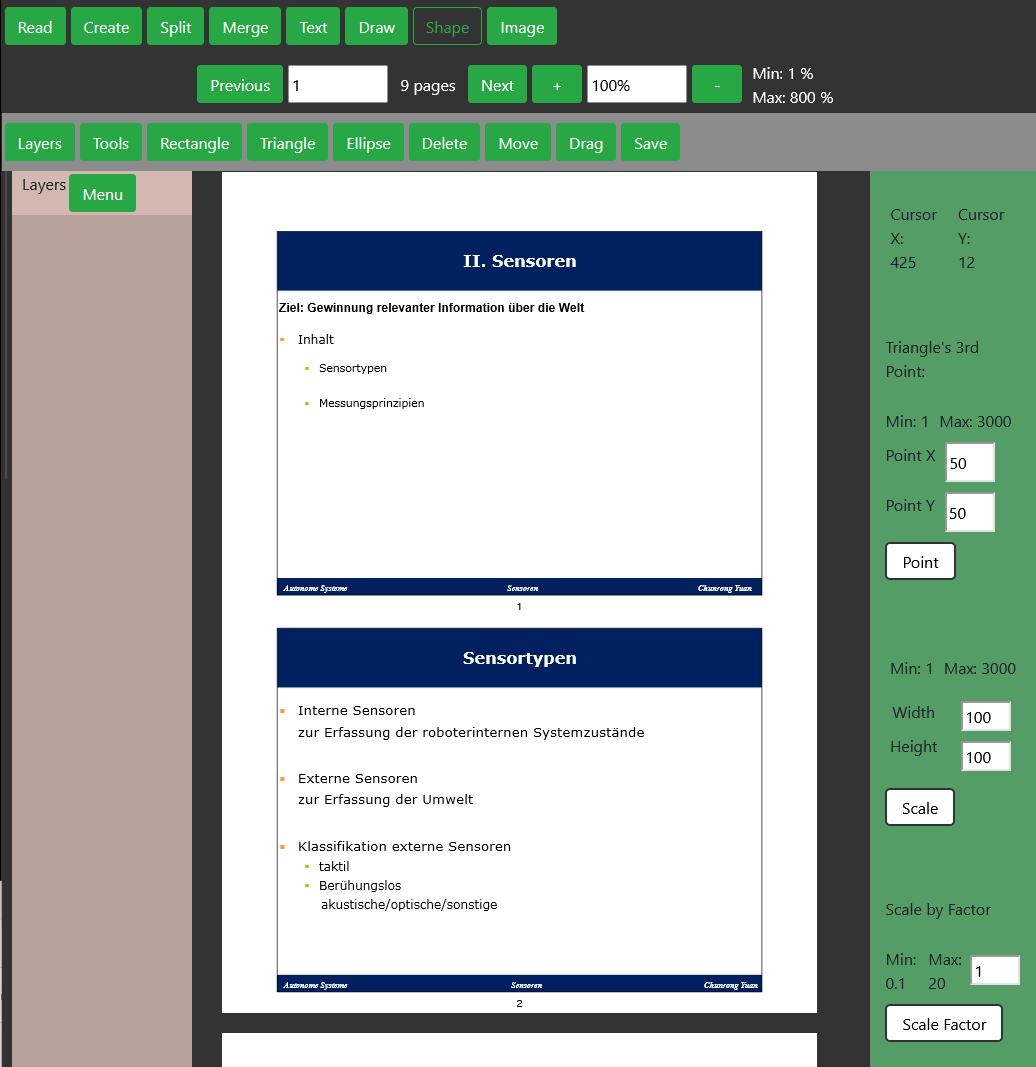
\includegraphics[width=1\textwidth]{"images/shaper.png"}
	\caption{Geometrieeditor der PDF Web App}
	\label{fig:shaper}
\end{figure}

\begin{figure}[!htbp]
	\centering
	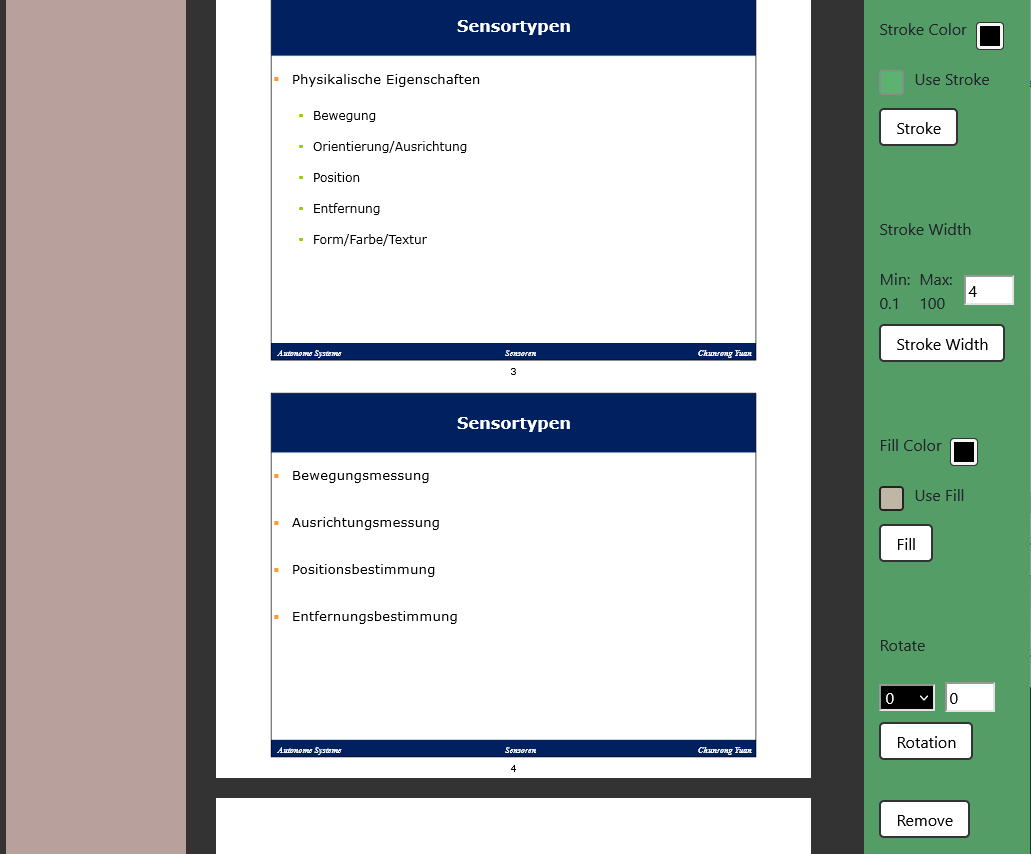
\includegraphics[width=1\textwidth]{"images/shaper2.png"}
	\caption{Mehr Tools des Geometrieeditors der PDF Web App}
	\label{fig:shaper2}
\end{figure}

Der Geometrietyp kann durch die Buttons Rectangle für Rechteck, Triangle für Dreieck oder Ellipse und einem oder mehreren Klicks auf eine PDF-Seite bestimmt werden. Jedem Shape wird eine orangene control box mehr oder weniger mittig hinzugefügt. Im Tools Seitenmenü des Geometrieeditors gibt es eine einzige Operation, die nur auf Dreiecke angewendet werden kann. Es handelt sich um die oberste Einstellung für die Position des dritten Punktes des Dreiecks. Hiermit kann der rechte Punkt der langen Spitze des default Dreiecks bearbeitet werden. Alle anderen Einstellmöglichkeiten können auf allen Geometrieelementen Rechteck, Dreieck und Ellipse arbeiten. Man hat 2 Möglichkeiten einen Shape zu skalieren. Zum einen kann man die Breite und Höhe unabhängig voneinander einstellen, was eine absolute Skalierung bedeutet, oder man verwendet den Skalierungsfaktor, der relativ vergrößert, genauso wie beim Drawer. Für die Shape Umrandungslinien kann man auf der einen Seite die Farbe inklusive Deckkraft und auf der anderen Seite die Breite der Linie justieren. Die Strichfarbe muss mit der Checkbox Use Stroke in Grün eingeschaltet sein, was sie beim ersten Öffnen des Editors auch ist. Deaktiviert man die Use Stroke Checkbox schaltet sich automatisch die Use Fill Checkbox an und umgekehrt. Man kann auch beide Checkboxen einschalten, aber nicht beide zusammen ausschalten. Ist Use Stroke Rosa, d.h. deaktiviert, und man wendet die Strichbreite an, dann hat Stroke Width keinen Effekt. Use Fill muss Grün sein, um die Füllfarbe anzuwenden. Bei Strich- und Füllfarbe wird ein wie in dem Writer und Drawer der gleiche color picker verwendet. Alle Shapes können mit absoluter Rotation rotiert werden. Die control boxes werden bei den Shapes mitgedreht. Zuunterst entfernt der Remove Button alle Geometrieelemente im geöffneten PDF. Der Screenshot \ref{fig:shaping} hebt mehrere bearbeitete Geometrieelemente hervor.

\begin{figure}[!htbp]
	\centering
	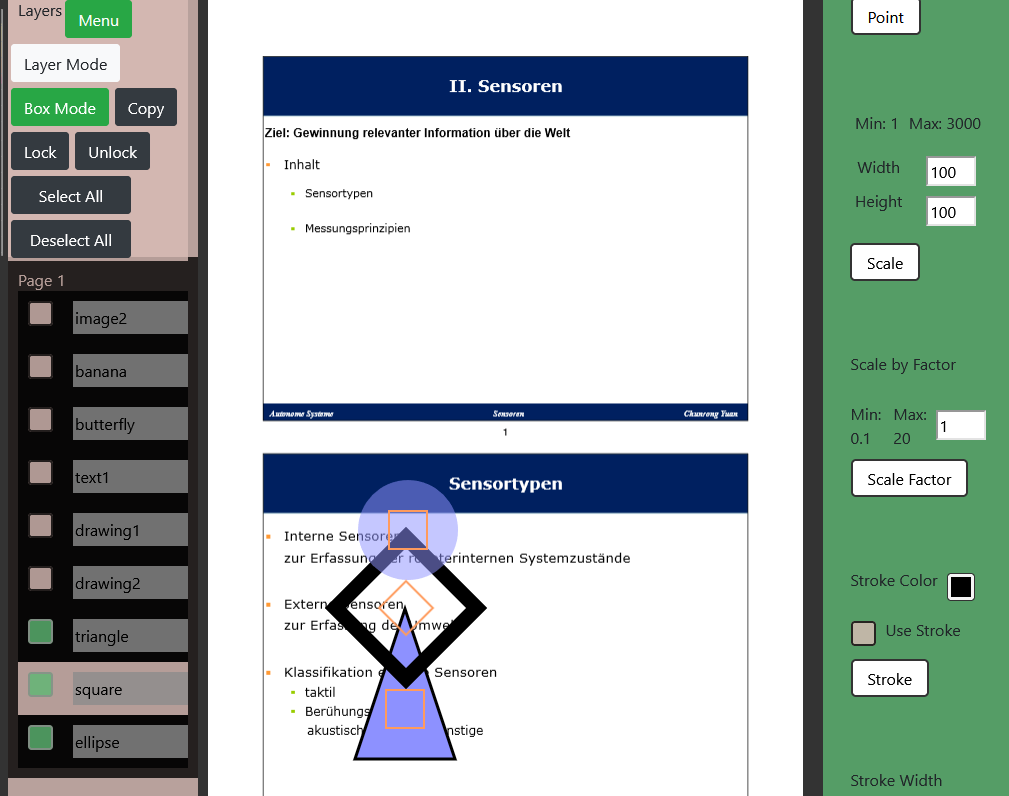
\includegraphics[width=1\textwidth]{"images/shaping.png"}
	\caption{Shapes im Geometrieeditor der PDF Web App}
	\label{fig:shaping}
\end{figure}


\subsubsection{Bilder einfügen}
Der Image Editor ist im Bild \ref{fig:images} dargestellt. 

\begin{figure}[!htbp]
	\centering
	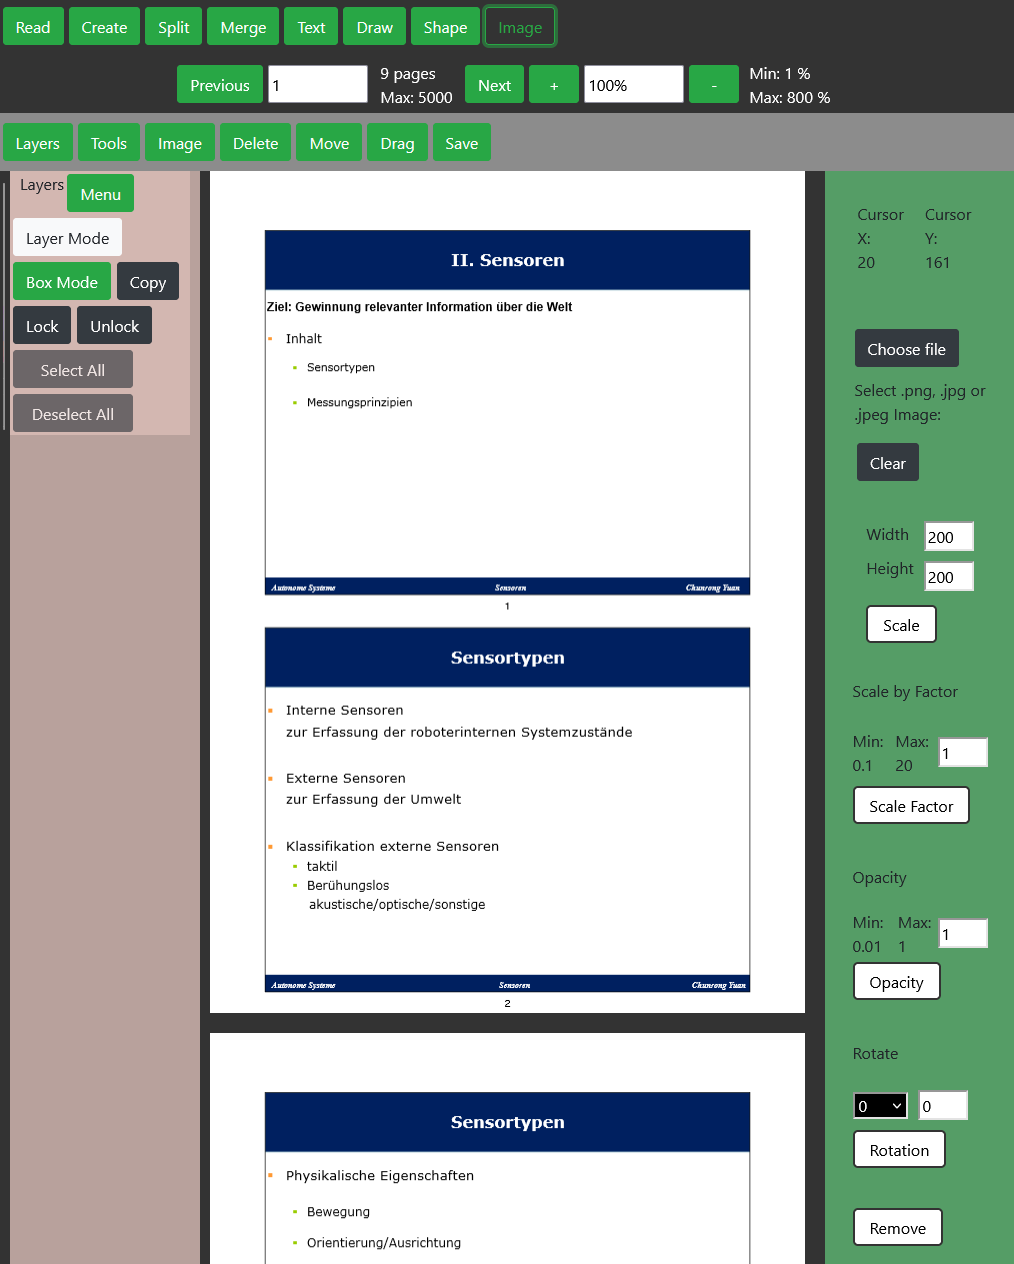
\includegraphics[width=1\textwidth]{"images/images.png"}
	\caption{Zeichnungen in der PDF Web App}
	\label{fig:images}
\end{figure}

Um ein Bild mit dem Image Button im Operations Bar hinzuzufügen, muss man erst ein Bild mittels dem schwarzen Choose file Button vom Dateisystem ausgewählt haben. Dann erscheint der Bildname wie im Writer bei einem benutzerdefinierten Font in der Liste unter Choose file. Man kann mehrere Bilder nacheinander im Dateidialog auswählen. Sie werden alle in der Liste untereinander angezeigt. Das zuletzt ausgewählte Bild wird zuunterst in der Liste angefügt und ausgewählt. Das Bild muss mit der runden Checkbox in Blau ausgewählt sein, um es mit Image und einem Klick auf eine Dokumentenseite auf dem PDF zu platzieren. Weiße Checkboxen stellen nicht ausgewählte Bilder dar. Mittels des dunkelgrauen Clear Buttons wird die Bildliste gelöscht. Die Bildselektionssektion funktioniert analog zum benutzerdefinierten Fontselektionsbereich im Writer. Bei der Bildplatzierung wird eine hellblaue control box dem Bildelement hinzugefügt. Ein Bild kann in Breite und Höhe unterschiedlich absolut skaliert werden und proportional mit einem Skalierungsfaktor relativ verkleinert bzw. vergrößert werden. Unter den Skalierungsoptionen kann man die Deckkraft eines Bildes bestimmen. Ebenfalls kann man ein Bild absolut drehen. Zuletzt können alle hinzugefügten Bildelemente im PDF mit dem Remove Button entfernt werden. Die Abbildung \ref{fig:imaging} zeigt den Image Editor in Aktion.

\begin{figure}[!htbp]
	\centering
	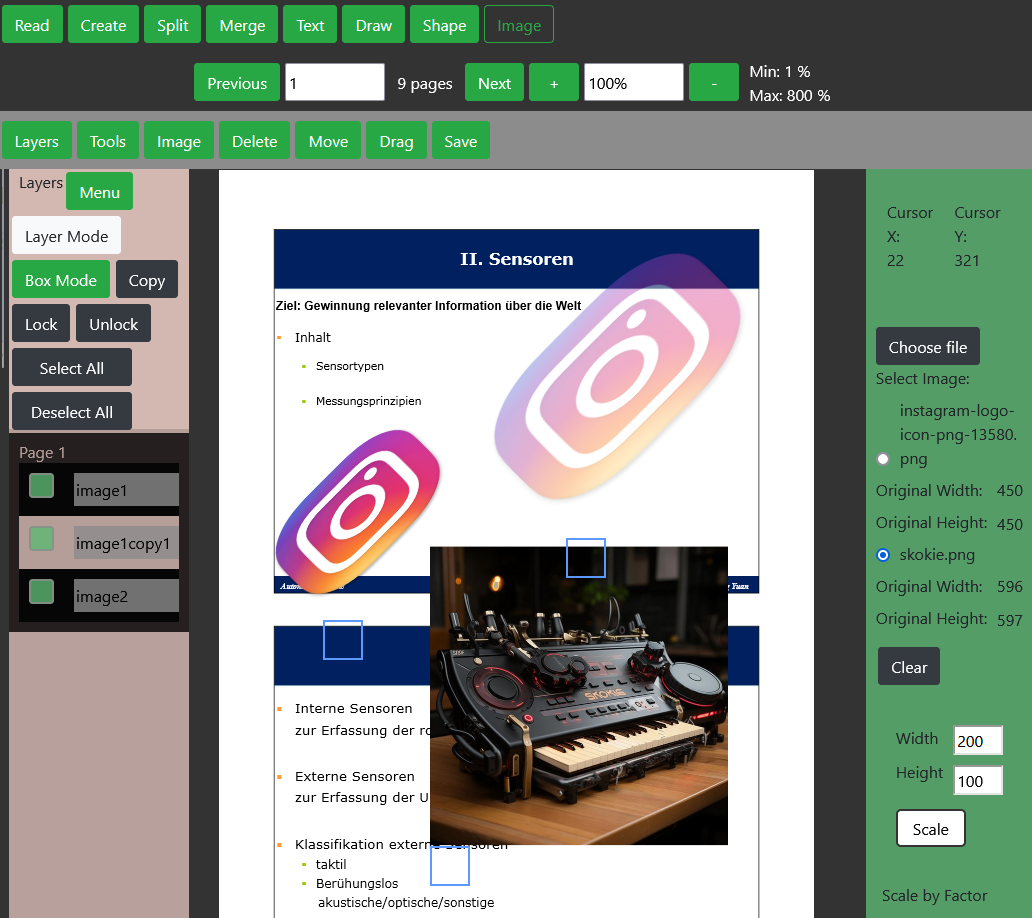
\includegraphics[width=1\textwidth]{"images/imaging.png"}
	\caption{Platzierte Bilder im Bildeditor der PDF Web App}
	\label{fig:imaging}
\end{figure}



\subsubsection{Ebenensteuerung}
Die in Abbildung \ref{fig:ebenenmenu} gezeigten Ebenenmenüschaltflächen lässen sich mit einem Klick auf Menu im rosa linken Ebenen Seitenmenü hervorholen oder verbergen. 

\begin{figure}[!htbp]
	\centering
	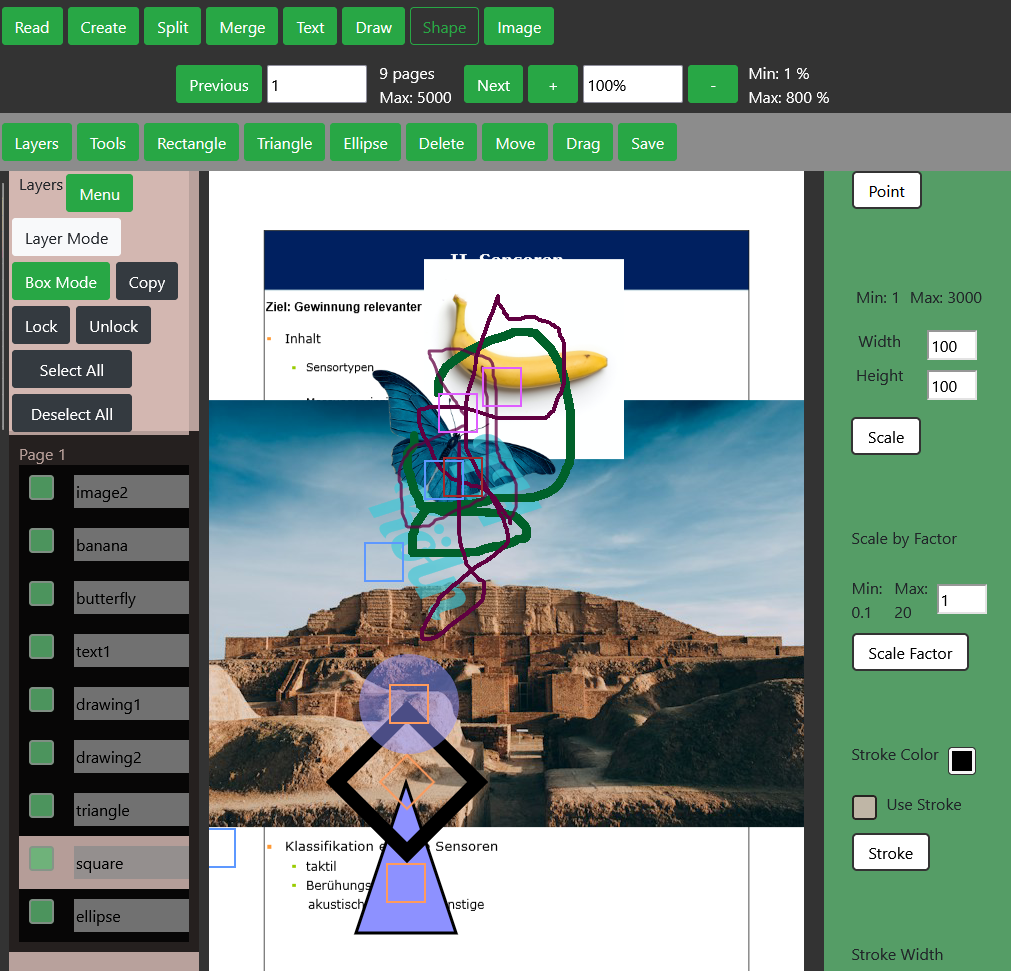
\includegraphics[width=1\textwidth]{"images/ebenenmenu.png"}
	\caption{Ausgeklapptes Ebenenmenu im Editor der PDF Web App}
	\label{fig:ebenenmenu}
\end{figure}

Standardmäßig sind die Schaltflächen eingeklappt. Fügt man ein Element unabhängig vom Typ einer PDF-Seite hinzu wird für dieses Element eine Ebene angelegt, die dann automatisch ausgewählt ist. Eine ausgewählte Ebene ist Rosa und eine abgewählte schwarz. Es können mehrere Ebenen ausgewählt werden. Wenn eine Ebene angelegt wird, bekommt sie einen Standardnamen gesetzt, der durch den Elementtyp und einem nummerischen Index gekennzeichnet ist. Der Standardname kann durch Tastatureingabe im grauen input field auf der Ebene überschrieben werden. Ebenen werden nach Seitenzahlen in einer schwarzen Box, die oberhalb mit der Seitenzahl gekennzeichnet ist, gruppiert. Dies verdeutlicht die Abbildung \ref{fig:ebenen}.   

\begin{figure}[!htbp]
	\centering
	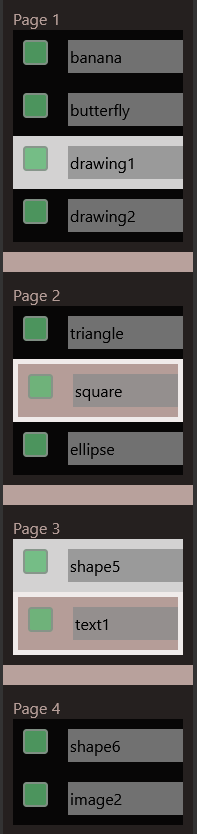
\includegraphics[width=0.3\textwidth]{"images/ebenen.png"}
	\caption{Ebenen mit Elementen allen Typs im Editor der PDF Web App}
	\label{fig:ebenen}
\end{figure}

Im Ebenenschaltflächenmenü kann man zwischen Box Mode und Layer Mode wechseln. Ist der Modus Button grün, so ist der betreffende Modus eingeschaltet. Hingegen ist ein ausgeschalteter Modus mit einem weißen Button versehen. Man kann nur entweder im Box Mode oder im Layer Mode sein, aber nicht in beiden Modi gleichzeitig. Mit dem dunkelgrauen Copy Button kann der Benutzer ausgewählte Ebenen kopieren. Folglich werden die beinhaltenden Elemente dubliziert. Wird eine Ebene kopiert, so wird an den Ebenennamen copy angehängt. Mit Lock und Unlock kann man Ebenen sperren bzw. entsperren. Eine gesperrte Ebene kann nicht verändert werden, d.h. keine Operationen können auf ihr beinhaltendes Element angewendet werden. Eine gesperrte unausgewählte Ebene ist weiß und eine gesperrte ausgewählte ist rosa mit weißer Umrandung, was auf Abbildung \ref{fig:ebenen2} verdeutlicht wird. 

\begin{figure}[!htbp]
	\centering
	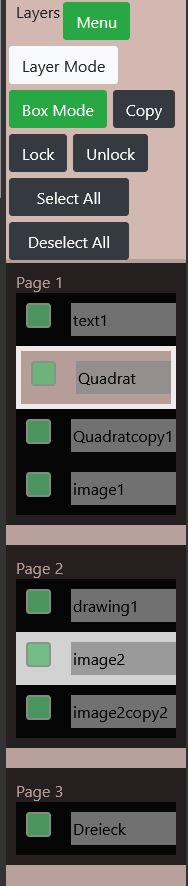
\includegraphics[width=0.3\textwidth]{"images/ebenen2.png"}
	\caption{Teilweise gesperrte Ebenen im Editor der PDF Web App}
	\label{fig:ebenen2}
\end{figure}

Die dunkelgrauen Select All und Deselect All Buttons stellen Auswahlfilter dar. Bewegt man die Maus auf die Buttons klappt sich ein Filtermenü auf, was im Bildausschnitt \ref{fig:filtermenu} gezeigt wird. 

\begin{figure}[!htbp]
	\centering
	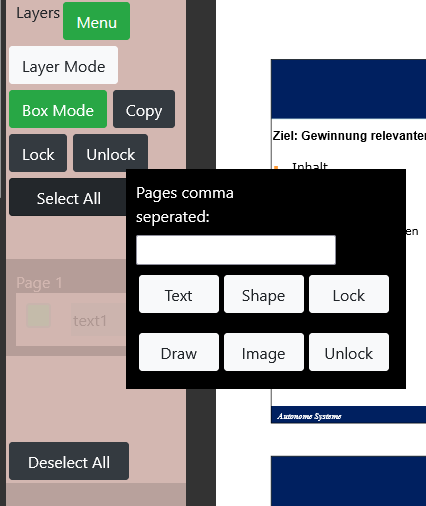
\includegraphics[width=0.6\textwidth]{"images/filtermenu.png"}
	\caption{Selection Filtermenü im Editor der PDF Web App}
	\label{fig:filtermenu}
\end{figure}

Bei Select All kann man mehrere Ebenen nach Seiten auswählen, nach Elementtyp und ob sie gesperrt oder nicht gesperrt sind, d.h. die Ebenen werden rosa markiert. Ist ein Filter aktiviert, werden die Buttons im Filtermenü grün. Bei weißen Buttons oder einer leeren Liste an Seiten ist kein Filter aktiviert. Bei der Seitenliste muss man die Seiten durch Komma trennen und sie müssen nicht in aufsteigender Reihenfolge angegeben werden. Die Filter werden mit einem Klick auf Select All angewendet. Ist kein Filter aktiviert, was der Standardzustand ist, so werden alle Ebenen mit Klick auf Select All ausgewählt. Deselect All hat die gleiche Funktionalität, nur dass die Filter zum Auswahl aufheben angewendet werden, d.h. Ebenen werden auf Schwarz gesetzt. Ein Klick auf Deselect All ohne Filter wählt alle Ebenen im Dokument ab. Im Bildausschnitt \ref{fig:filtering.} ist ein Beispiel abgebildet. Laut des Beispiels würde die Auswahl auf allen ungesperrten Textelementen auf Seite 1 und 2 aufgehoben werden. 


\begin{figure}[!htbp]
	\centering
	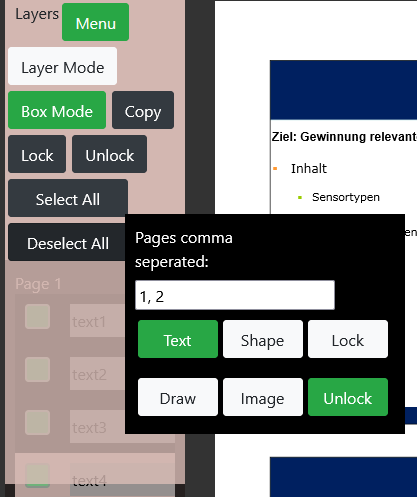
\includegraphics[width=0.6\textwidth]{"images/filtering.png"}
	\caption{Deselection Filtermenü mit aktivierten Filtern im Editor der PDF Web App}
	\label{fig:filtering}
\end{figure}

Die Reihenfolge der Elemente in der z-Achse kann über die Ebenen gesteuert werden. Man kann ein einzelnes Element mit gedrückter Maustaste auf eine andere Ebene verschieben, um die Position zu ändern, wie Elemente übereinander liegen. Dabei ändert sich das Maussymbol. Man muss zwecks Verschiebung in der z-Achse auf den Ebenen Namen oder auf die rosa Fläche initial die Maus drücken und dann ziehen. Dabei kann man sogar ein Element in eine andere Ebenengruppe ziehen, sodass das Element auf der entsprechenden Seite erscheint. Links neben jedem Ebenennamen ist eine grüne Checkbox abgebildet. Wenn man sie abwählt, färbt sie sich rosa und das Element wird samt control box unsichtbar. Dann können ebenfalls keine Operationen angewendet werden. Ein erneuter Klick auf die Ebenencheckbox schaltet sie wieder in Grün ein und das Element wird auf der Seite erneut sichtbar. 


\subsubsection{Arbeiten im Layer Mode}
Ich habe bisher alle Operationen im Box Mode beschrieben. Es gibt außerdem den Layer Mode, den man im Ebenenschaltfächenmenü aktivieren kann. Im Layer Mode kann der Benutzer ein oder mehrere Ebenen auf allen PDF-Seiten selektieren und dann Move, Delete und alle Operationen im Tools Seitenmenü auf sie anwenden. Um dies umzusetzen, muss man bei Tools seine gewünschte Einstellung machen und auf den jeweiligen weißen Button klicken. Sofort werden die Einstellungen auf die selektierten Ebenen mit einem einzigen Klick angewendet. Es ist nicht mehr nötig in irgendeine control box zu klicken. Dabei sind die Einstellungen in Tools elementspezifisch. Wird beispielsweise eine Tools-Einstellung des Writers auf eine Shape Ebene angewendet, wird sie ignoriert. Ist dabei auch noch eine Textebene ausgewählt, so wird die Operation nur auf die Textebene angewendet. Delete und Move können in jedem Editormodul im Layer Mode auf alle Elementtypen angewendet werden. Vor allem bei Move muss man in einer control box, dessen Ebene ausgewählt ist, die Maus drücken und auf eine gewünschte Stelle auf der PDF-Seite ziehen. Alle anderen Ebenen, die zusätzlich ausgewählt wurden, werden mit gleichem proportionalem Abstand zueinander um die gewünschten Verschiebungskoordinaten verschoben. Wenn die control box losgelassen wird, springen die Elemente an die jeweiligen Stellen. Ob man lieber im Box Mode oder Layer Mode arbeitet, ist Geschmackssache. Jeder Modus bringt seine Vor- und Nachteile mit sich, die ich im Kapitel Diskussion und Kritik aufzeigen werde.